%%% Local Variables: 
%%% mode: latex
%%% TeX-master: t
%%% End: 

\documentclass[12pt]{article}
\usepackage{graphicx}
\usepackage[T1]{fontenc}		% F�r svenska bokst�ver
\usepackage[swedish]{babel}
\usepackage{listings}


\title{TDTS07 Lab Report 1}
\author{Nora Bj�rklund and Christopher Hallberg}
\begin{document}
\maketitle

\section{Exercise}
\textbf{A<> P.s3} was not satisfied since s0 just can stay in its own state since there are no invariants, while \textbf{E<> P.s3} is satisfied since the system \textit{can} end up in state s3. Once the system starts from the initial state it will never go back to it. 
\section{Fischer part I}
\begin{table}[h]
  \centering
  \begin{tabular}{|c|c|c|}
    \hline
    n  & Seconds to finish \\
    \hline
    8  & < 1 \\
    9  & 4 \\
    10 & 16 \\
    11 & 60 \\
    12 & 240 (?) \\
    \hline
  \end{tabular}
  \caption{Table for n instances of Fischer's mutual exclusion protocol }
  \label{tab:n_fischer}
\end{table}
\section{Fischer part II}

\section{Traffic Light Controller}
The traffic light controller is implemented with a process P, and a timer. The timer have two states, one where it can let cars coming from north or south drive and one state when cars from east and west can drive and it changes when an invariant c is more than a certain number c1. When the timer changes state a synchronisation call is set, the invariant c is set to 0 and boolean assignments that north-south or west-east can drive or not.

% Bild p� timer
\begin{figure}[h]
  \centering
  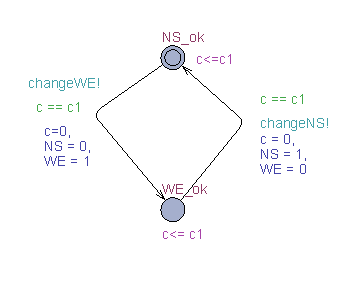
\includegraphics[width=0.7\textwidth]{timer.png}
  \caption{Timer}
  \label{fig:timer}
\end{figure}

The process P starts in an initial state, Red\_no\_car, where the system have no waiting cars. Incoming cars have a signal i, and if that signal is greator than or equal to 3 then the car is coming from the north or the south. If it is less than or equal to 2 then it is a car from either west or east. The  variable i is then used as an invariant placing the system in either state wait\_WE (waiting car from west or east) or in wait\_NS. Here the system synchronizes with the timer, so if a car from east is waiting for green then it has to wait for changeWE! to occur. When synched with the timer the system is in a state called green which represents that the car is given green and dissapears, we then once more wait to synchronize with the timer bringing the system back to the initial state. We have then created four instances of the process called N, S, W and E to represent the four directions.

% Bild p� P 
\begin{figure}[h]
  \centering
  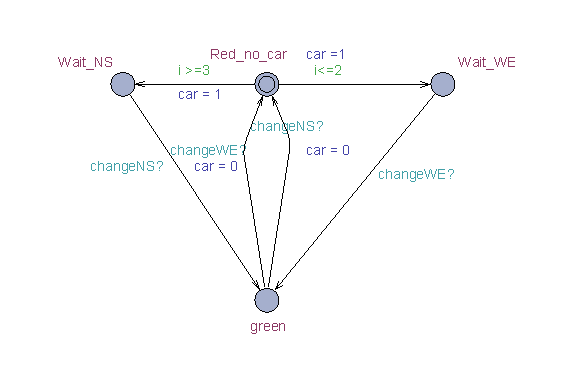
\includegraphics[width=0.7\textwidth]{trafficlight.png}
  \caption{Process P}
  \label{fig:p}
\end{figure}

We verify the following on the system:
\begin{itemize}
\item $A[]$ not deadlock, check that the system does not deadlock
\item $E<>$ X.green, check that the system eventually has the ability to end up in X.green (we do this for all directions so insert either N, S, W or E instead of X).
\item $E<>$ E.Wait\_WE, checks that the system eventually could end up in E.Wait\_WE, we do the same for the other directions, though N and S uses Wait\_NS instead of Wait\_WE.
\item $W.car -->W.green$, checks that if we are in state W.car will transition to W.green (if true that means a waiting car will be given green)
\item $S.car -->S.green$ 
\item $A[]$ not ((N.green or S.green) and (W.green or E.green)), if false then we can give a car from the north and the west green at the same time. 
\end{itemize}
\section{Alternating Bit Protocol}
The alternating bit protocol consists of three processes, a sender, a reciever and an unreliable channel and it works as explained in the lab tutorial. 
% Bild p� alla systemen :D

\begin{figure}[h!]
  \centering
  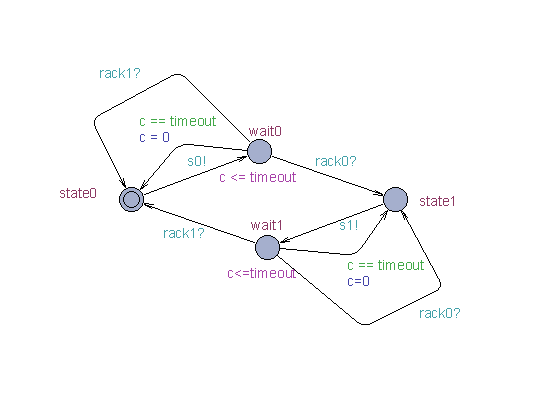
\includegraphics[width=0.7\textwidth]{sender.png}
  \caption{Sender}
  \label{fig:s}
\end{figure}

\begin{figure}[h!]
  \centering
  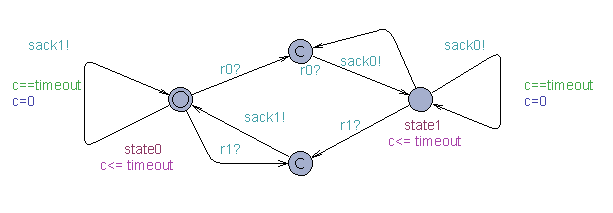
\includegraphics[width=0.7\textwidth]{reciever.png}
  \caption{Reciever}
  \label{fig:r}
\end{figure}

\begin{figure}[h!]
  \centering
  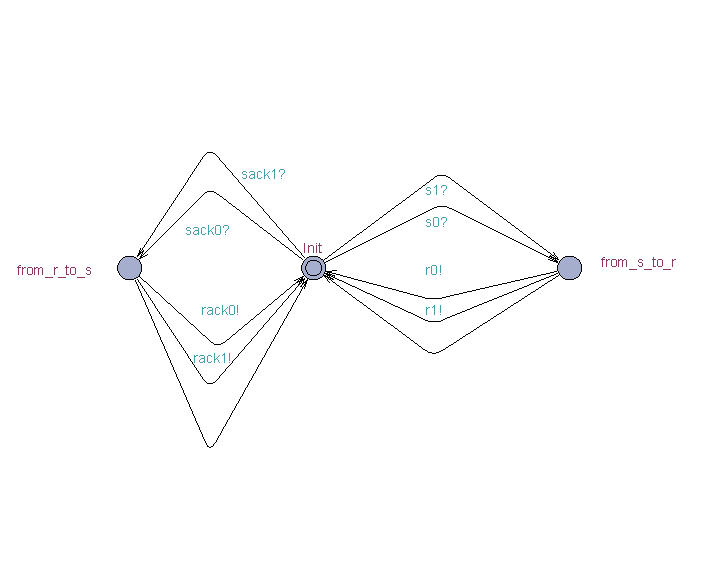
\includegraphics[width=0.7\textwidth]{unrel_chan.png}
  \caption{Unreliable channel}
  \label{fig:unrel_chan}
\end{figure}

The system was verified for the following statements:
\begin{itemize}
\item$ E<> U.from\_r\_to\_s$, the unreliable channel might eventually end up in state from\_r\_to\_s, is a true statement.
\item $S.state0-->R.state1$, given that the sender is in state0 the reciever will eventually go to its state1.This is a false statement since the unrelaiable channel can lose messages.
\item $S.state1-->R.state0$, this is also a false statement (same explanation as above)
\item $A[] not deadlock$, the system will never deadlock (true in the system)
\end{itemize}
\end{document}
